\documentclass[conference]{IEEEtran}
\IEEEoverridecommandlockouts
\usepackage{cite}
\usepackage{amsmath,amssymb}
\usepackage{graphicx}
\usepackage{xcolor}
\usepackage{listings}
\usepackage{url}
\usepackage{booktabs}

\lstdefinestyle{ccode}{language=C,basicstyle=\ttfamily\scriptsize,breaklines=true,
 frame=single,numbers=left,numberstyle=\tiny\color{gray},
 keywordstyle=\color{blue!70!black},commentstyle=\color{green!40!black},
 showstringspaces=false,columns=fullflexible}
\lstdefinestyle{asm}{basicstyle=\ttfamily\scriptsize,breaklines=true,frame=single,
 numbers=none,commentstyle=\color{gray},showstringspaces=false,columns=fullflexible}

\begin{document}

\title{AI-Driven Reverse Engineering of Compiled Software:\\
How Large Language Models Are Changing the Threat Model\\
for Software Confidentiality}

\author{
\IEEEauthorblockN{Charbel J. Estephan}
\IEEEauthorblockA{Dept.\ of Computer and Communications Engineering\\
Notre Dame University -- Louaize\\
Zouk Mosbeh, Lebanon}
\and
\IEEEauthorblockN{[Second Author]}
\IEEEauthorblockA{Dept.\ of Computer and Communications Engineering\\
Notre Dame University -- Louaize\\
Zouk Mosbeh, Lebanon}
}

\maketitle

\begin{abstract}
Reverse engineering of compiled software has always threatened the
confidentiality of proprietary code, embedded secrets, and licensing logic, but
it demanded scarce expert skill. Large language models are removing that barrier.
Tools that decompile binaries end to end and recover names, types, and
natural-language descriptions from stripped executables turn a slow expert task
into a fast, automated one, lowering the skill and time an attacker needs to
understand and crack software. This report examines AI-driven reverse engineering
as an emerging offensive capability. We define the technology and why it is
spreading, map the assets it endangers and who owns them, analyze its core
vulnerabilities against the Confidentiality-Integrity-Availability triad and
profile the attacker with the Method-Opportunity-Motive framework, and, as our
main focus, explain why the industry cannot easily solve the problem. To ground
the analysis in evidence rather than assertion, we conduct a small reproducible
measurement study: four sample programs, each hiding a secret value or a secret
algorithm, are protected at three levels and assessed for how much of their
purpose and secret survive. Across all four, obfuscation cuts mean purpose
recovery from 5.0 to 2.0 out of 5 but cuts secret recovery only from 5.0 to 3.5,
because the defining data constants survive transformations that scramble control
flow. That gap is the crux of the industry's difficulty: hiding what a program is
costs little, hiding the data an AI can read costs a great deal, and AI capability
is improving faster than affordable defenses.
\end{abstract}

\begin{IEEEkeywords}
AI-driven cyberattacks, large language models, reverse engineering, software
confidentiality, code obfuscation, threat modeling, C-I-A triad
\end{IEEEkeywords}

\section{Introduction and Technological Overview}
Software ships to users as compiled machine code. For decades that machine code
has been readable to a determined expert with a disassembler and a decompiler,
which is why reverse engineering sits behind software piracy, intellectual
property theft, malware analysis, and vulnerability discovery. What held the
threat in check was skill: reading decompiled assembly, reconstructing lost names,
and untangling optimized control flow took years of training and many hours per
target. That gate is now being removed by artificial intelligence, which is why a
long-standing risk belongs on a list of modern, rapidly evolving security
domains.

\textbf{What the technology is.} AI-driven reverse engineering is the use of
machine learning, and large language models (LLMs) in particular, to automate the
understanding of compiled programs. The pipeline is familiar; the automation is
new. A disassembler recovers instructions; a decompiler lifts them into C-like
pseudocode; and an LLM then reads that output and explains it, renames variables
and functions, recovers data structures, or rewrites it into clean source.
LLM4Decompile, an open model series trained specifically to decompile binaries,
reports results that surpass both GPT-4 and the Ghidra decompiler on standard
benchmarks~\cite{llm4decompile}. A parallel line of work recovers the symbols that
stripping removes: ReSym recovers variable names and data structures by combining
an LLM with program analysis~\cite{resym}, and other systems recover function
names from stripped binaries~\cite{gennm,funcname}. Empirical studies now measure,
rather than assume, how capable these models are at understanding real stripped
code~\cite{howfar,empirical}.

\textbf{A concrete pipeline.} In practice an attacker chains the stages into a
near-automatic workflow. The target binary is loaded into a decompiler such as
Ghidra~\cite{ghidra}, which produces pseudocode. That pseudocode, often ugly and
missing names, is handed to an LLM with a simple instruction: explain this
function, rename the variables, or rewrite it as clean C. A name-recovery model
labels the stripped functions so the attacker knows which to read first. For a
protected target, an automated deobfuscation or symbolic-execution pass can
simplify the control flow before the model sees it~\cite{angr,udupa}. Each stage
used to be a specialist skill; now each is a tool call, and the attacker's main
job is to point the pipeline at the right function.

\textbf{The four artifacts that leak intent.} It helps to name what the AI reads,
because every protection and every weakness discussed later targets one of these.
First, \emph{symbols}: the names of functions and variables, a labelled map of the
program when present. Second, \emph{strings}: readable text such as error messages
and prompts, which announce intent in plain language and are the fastest signal an
analyst has. Third, \emph{data constants}: the keys, thresholds, and small
arithmetic baked into instructions, which define what a check accepts or what an
algorithm computes. Fourth, the \emph{control-flow graph} (CFG): the shape of
loops and branches, which when it mirrors the source lets a reader follow the
logic. Human and AI analysts alike reconstruct a program by recovering these four
things. Defenders try to remove them; AI makes the removal harder to rely on.

\textbf{Why it is a new frontier.} Traditional computer security often assumes a
bounded, defended perimeter with a defender watching. Shipped software is the
opposite: the artifact is in the attacker's hands, on their machine, with
unlimited time and no network defender in the loop. The only protection is how
hard the binary is to understand. For decades that difficulty was a reliable
deterrent because expert reverse-engineering talent was scarce and slow. AI breaks
that assumption. When understanding becomes fast, cheap, and scalable, every
secret shipped inside a binary, every key, license check, and proprietary
algorithm, becomes far more exposed than its owner assumed when they compiled it.
The capability, not the artifact, has changed, and that is what makes this a
current security frontier rather than settled history.

\section{Landscape of Assets and Value}
The value at risk in a binary is not the file itself but what the file reveals or
enables once understood.

\textbf{Key assets.}
\begin{itemize}
\item \textbf{Proprietary algorithms and IP.} Trading strategies, codecs, ranking
or pricing logic, and signal-processing routines are often a company's core
advantage, compiled into a product that customers run.
\item \textbf{Licensing and DRM logic.} The code that decides whether a copy is
licensed. Understanding it enables key generators, patches, and piracy.
\item \textbf{Embedded secrets.} Hardcoded keys, API tokens, credentials, and
magic constants. Studies of real software repeatedly find secrets baked into
shipped binaries and firmware.
\item \textbf{Firmware and device logic.} The control software of IoT devices,
vehicles, and medical equipment, where understanding the binary is the first step
to finding exploitable flaws.
\end{itemize}

\textbf{Concrete domains.} The abstract assets map onto familiar industries. In
gaming, anti-piracy systems protect both the license check and the game logic, and
the long history of DRM being cracked within days of release shows how motivated
and well resourced the attacker side is. In mobile apps, the shipped package
contains client-side logic that attackers repackage, clone, or strip of ads. In
the Internet of Things and embedded devices, firmware extracted from a chip has
repeatedly been found to contain hardcoded credentials and keys, turning one
cracked device into a master key for an entire product line. In automotive and
medical devices, the control firmware is the first target for anyone hunting
safety-critical flaws. Each domain ships a binary whose understanding unlocks
something valuable.

\textbf{Who owns them and why they are targets.} Software vendors and game studios
own licensing and IP and are targeted for piracy and competitive intelligence.
Embedded and device manufacturers own firmware and are targeted for vulnerability
discovery and counterfeiting. Security researchers and malware authors both target
any binary, the former to find flaws, the latter to learn from and weaponize them.
The common thread is that the owner has lost physical control of the artifact: once
the binary is distributed, its confidentiality rests entirely on the difficulty of
reverse engineering, which is precisely the difficulty that AI is eroding. The
value at stake scales with the asset, from a single stripped ad in a free app to
the entire intellectual property of a trading firm or the safety of a connected
vehicle.

\section{Threat and Vulnerability Analysis}
\subsection{Core Vulnerabilities}
AI-driven reverse engineering does not exploit a software bug; it exploits
structural properties of compiled software and amplifies them.

\textbf{V1: Compiled code inherently leaks recoverable artifacts.} A binary is not
a secret. To run, it must contain real instructions, and it typically also carries
the four artifacts named above. An analyst reads intent from them, and nothing
about compilation removes them by default.

\textbf{V2: LLMs automate and scale the recovery.} The historical defense was not
that the artifacts were absent but that reading them was slow expert work. LLMs
attack exactly this. They decompile end to end~\cite{llm4decompile}, invent the
names that stripping removed~\cite{gennm,funcname,resym}, and summarize a
function's purpose in natural language~\cite{howfar}. The skill barrier that
limited the threat population collapses, and the work parallelizes.

\textbf{V3: Current defenses are delay, not denial.} Obfuscation, the standard
defense, raises cost but does not eliminate recovery. Flattened control flow is
simplified by automated deobfuscation and symbolic execution~\cite{angr,udupa};
packers are undone by running the program and dumping memory~\cite{rolles}; and
even heavy virtualization is lifted by recovering its interpreter. Worse, as our
measurement study in Section~\ref{sec:study} shows, lightweight obfuscation leaves
the secret data constants in place even when it hides program structure.

\subsection{Exploitation in Practice}
These weaknesses are exploited along two paths. The first is direct cracking. An
attacker locates the license or integrity check, understands it with AI-assisted
decompilation, and then patches the binary or forges a key. The decades-long
pattern of game DRM being defeated shortly after release shows the economic pull,
and AI lowers the skill and time each new crack requires. The second path is
intelligence and exploitation. A malware analyst or an adversary uses the same
pipeline to summarize thousands of functions, find the one that handles secrets or
parses untrusted input, and focus effort there, accelerating both defensive triage
and offensive vulnerability discovery. In both paths the model does not break
cryptography or find a zero day on its own; it removes the comprehension
bottleneck that used to protect the code, which is enough to change the economics
of the attack.

\subsection{Mapping to the C-I-A Triad}
\textbf{Confidentiality} is the property most directly compromised. The entire
threat is about reading what the owner wished to keep secret: algorithms, keys, and
licensing logic. AI-driven RE is, at its core, a large-scale confidentiality
attack on shipped code.

\textbf{Integrity} is compromised as a direct consequence. Once an attacker
understands a license check or an integrity routine, they can patch it, forge keys,
or tamper with program behavior. Understanding enables modification, so a
confidentiality break becomes an integrity break.

\textbf{Availability} is affected indirectly. Pirated or cracked software undermines
the commercial availability of the legitimate product and its update channel, and
vulnerabilities discovered through AI-assisted RE can later feed attacks that take
systems down. Availability is the least direct of the three but not absent.

\subsection{Attacker Profile (M-O-M)}
\textbf{Method.} LLM-augmented decompilers and name-recovery
models~\cite{llm4decompile,resym,gennm}, automated deobfuscation and symbolic
execution~\cite{angr,udupa}, and dynamic unpacking~\cite{rolles}, chained into
pipelines that need little expert input.

\textbf{Opportunity.} Maximal. The binary is distributed to the attacker, who runs
it on their own hardware with unlimited time, no network defender, and free or
cheap tools. Shipping software is handing the attacker the artifact.

\textbf{Motive.} Piracy and license circumvention, intellectual-property and
algorithm theft, competitive intelligence, vulnerability discovery for later
exploitation, and malware development and analysis.

\textbf{Why M-O-M matters here.} All three factors move in the attacker's favor at
once. Opportunity was always maximal for shipped software, and motive has always
existed; what historically limited the threat was method, the skill and time to
carry it out. AI raises the method factor for a huge population of would-be
attackers, so a threat that was previously gated by expertise becomes broadly
accessible. That shift, from an expert-only method to a commodity one, is the
precise mechanism by which an old risk becomes a modern one.

\section{Original Measurement Study: What Protection Actually Hides}\label{sec:study}
The threat analysis rests on a claim that deserves evidence: that lightweight
protection hides a program's structure far more effectively than it hides the
secret data inside it. To test this directly, and to go beyond summarizing others'
work, we built a small, fully reproducible testbed. All code, build scripts, and
results are in a public repository so the numbers below can be regenerated from
source.

\subsection{Method}
We wrote four small C programs with behavior we fully control, so the ``right
answer'' an analyst seeks is always known.
\begin{itemize}
\item \textbf{P1}, a license validator (XOR-sum of the password compared to a
magic constant). Protects a secret \emph{value}.
\item \textbf{P2}, a Collatz stopping-time computer ($3n{+}1$). Protects a secret
\emph{algorithm}.
\item \textbf{P3}, a djb2 hash key check (seed \texttt{5381}). Protects a named
algorithm and its constants.
\item \textbf{P4}, an eight-digit serial validator with a mod-10 check digit.
Branch-heavy logic.
\end{itemize}
Each program was compiled at three cumulative protection levels: \textbf{L0}
(\texttt{-O0}, symbols kept); \textbf{L1} (\texttt{-O2} then \texttt{strip -s});
and \textbf{L2}, a source-level rewrite applying control-flow flattening, opaque
predicates, and string encryption, then \texttt{-O2} and stripping.
Listing~\ref{lst:flatten} shows the flattening pattern: the natural loop becomes a
dispatcher over a state variable, guarded by an opaque predicate \texttt{OP} that
is always true, with a dead sink state that never runs. We verified that all three
levels of every program produce identical output, including the known fact that
the Collatz stopping time of 27 is 111 steps.

\begin{lstlisting}[style=ccode,caption={Control-flow flattening at L2 (P1, abridged).},label={lst:flatten}]
#define OP(x) ((((unsigned)(x)*(unsigned)(x) \
               - (unsigned)(x)) & 1u) == 0u) /* always true */
int state=0, acc=0; size_t i=0;
for (;;) switch (state) {
  case 0: if (OP(len)){acc=0;i=0;state=1;} else state=99; break;
  case 1: state=(i<len)?2:3; break;
  case 2: acc+=(pw[i]^0x5A); i++; state=OP(i)?1:99; break;
  case 3: result=(acc==0x3F7); state=100; break;
  case 99: acc^=0xFFFF; state=1; break; /* dead sink */
  case 100: return result;
}
\end{lstlisting}

We measured three things per binary: objective static indicators
(\texttt{nm} symbol count, \texttt{strings} count, presence of the plaintext
secret output); an objective control-flow complexity proxy (counts of conditional,
unconditional, and indirect jumps); and an analyst recovery score on a 0--5 scale
for program purpose and for the embedded secret, assigned from a reading of the
disassembly. We note a validity caveat: the analyst was an LLM, and a similar model
assisted in producing the obfuscated code, so the analyst is not fully blind. The
static and complexity numbers are script-derived and model-independent, and anchor
the subjective scores; independent replication with a separate model and with human
analysts timed by hand is the right next step.

\subsection{Results}
Table~\ref{tab:static} reports the static indicators. Stripping (L1) removes every
symbol, and string encryption (L2) is the only step that removes the plaintext
secret output. Table~\ref{tab:cfg} shows the complexity proxy: flattening at L2
raises every count, most clearly the indirect jumps, because the compiler lowers
the state dispatcher to a jump table. Table~\ref{tab:recovery} and
Fig.~\ref{fig:recovery} report recovery. The trend is identical across all four
programs: obfuscation cuts mean purpose recovery from 5.0 to 2.0, but cuts mean
secret recovery only from 5.0 to 3.5.

\begin{table}[t]
\caption{Static protection indicators per program and level.}
\label{tab:static}
\centering\footnotesize
\begin{tabular}{@{}llcccc@{}}
\toprule
\textbf{Prog} & \textbf{Level} & \textbf{Symbols} & \textbf{Strings} & \textbf{Secret str.} & \textbf{Size (B)} \\
\midrule
P1 & L0 & 33 & 80 & yes & 16088 \\
P1 & L2 & 0  & 52 & no  & 14472 \\
P2 & L0 & 33 & 79 & n/a & 16096 \\
P2 & L2 & 0  & 46 & n/a & 14472 \\
P3 & L0 & 32 & 79 & yes & 16040 \\
P3 & L2 & 0  & 47 & no  & 14472 \\
P4 & L0 & 33 & 81 & yes & 16080 \\
P4 & L2 & 0  & 53 & no  & 14472 \\
\bottomrule
\end{tabular}
\end{table}

\begin{table}[t]
\caption{Control-flow complexity (mean per binary, four programs).}
\label{tab:cfg}
\centering\footnotesize
\begin{tabular}{@{}lccc@{}}
\toprule
\textbf{Level} & \textbf{Cond.\ branches} & \textbf{Uncond.\ jumps} & \textbf{Indirect jumps} \\
\midrule
L0 (none)       & 11.3 & 14.5 & 6.8 \\
L1 (strip+opt)  & 12.0 & 11.8 & 6.8 \\
L2 (obfuscated) & 15.0 & 18.0 & 8.0 \\
\bottomrule
\end{tabular}
\end{table}

\begin{table}[t]
\caption{Analyst recovery scores (0--5).}
\label{tab:recovery}
\centering\footnotesize
\begin{tabular}{@{}llcc@{}}
\toprule
\textbf{Program} & \textbf{Level} & \textbf{Purpose} & \textbf{Secret} \\
\midrule
P1 & L0 & 5 & 5 \\ P1 & L2 & 2 & 3 \\
P2 & L0 & 5 & 5 \\ P2 & L2 & 2 & 4 \\
P3 & L0 & 5 & 5 \\ P3 & L2 & 2 & 4 \\
P4 & L0 & 5 & 5 \\ P4 & L2 & 2 & 3 \\
\midrule
\textbf{Mean} & L0 & \textbf{5.0} & \textbf{5.0} \\
\textbf{Mean} & L1 & \textbf{4.0} & \textbf{5.0} \\
\textbf{Mean} & L2 & \textbf{2.0} & \textbf{3.5} \\
\bottomrule
\end{tabular}
\end{table}

\begin{figure}[t]
\centering
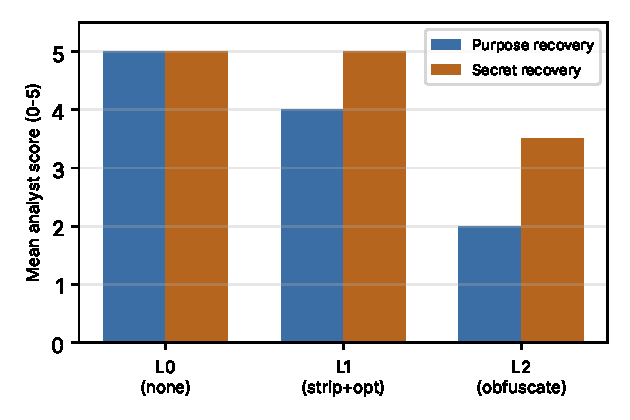
\includegraphics[width=0.80\columnwidth]{recovery.pdf}
\caption{Mean recovery of program purpose versus secret as protection increases.
Obfuscation collapses purpose recovery but leaves the secret partially exposed
because data constants survive.}
\label{fig:recovery}
\end{figure}

\subsection{Why the Secret Survives: A Disassembly Walkthrough}
The gap is clearest at the instruction level. At L0, the Collatz routine (P2)
disassembles to a short linear loop (Listing~\ref{lst:asm-l0}) in which the parity
test (\texttt{and \$0x1}), the halving (\texttt{shr \$1}), the $3n{+}1$ step
(\texttt{add \%rax,\%rax; add \%rdx,\%rax; add \$0x1}), and the termination
(\texttt{cmpq \$0x1}) are all explicit. At L2 (Listing~\ref{lst:asm-l2}), the
flattened dispatcher has become an indirect jump through a jump table
(\texttt{notrack jmp *\%rsi}), the dead sink shows as a never-taken
\texttt{add \$0xdead}, and function boundaries are gone, so program purpose is hard
to state. Yet \texttt{lea (\%rax,\%rax,2)} still computes $3n$ in plain sight, and
for P1 the constants \texttt{0x3F7} and \texttt{0x5A} remain in the instruction
stream. The structure is destroyed; the data is not.

\begin{lstlisting}[style=asm,caption={P2 at L0: the algorithm is explicit.},label={lst:asm-l0}]
and  $0x1,%eax      ; parity test (n odd?)
shr  $1,%rax        ; n = n/2
add  %rax,%rax      ; 2n
add  %rdx,%rax      ; 2n+n = 3n
add  $0x1,%rax      ; 3n+1
cmpq $0x1,-0x18(%rbp); while (n != 1)
\end{lstlisting}

\begin{lstlisting}[style=asm,caption={P2 at L2: structure hidden, arithmetic survives.},label={lst:asm-l2}]
cmp  $0x9,%ecx          ; dispatch on state
lea  (%rax,%rax,2),%rax ; 3n  <-- survives
add  $0x1,%rax          ; +1
add  $0xdead,%rdx       ; dead sink (never runs)
notrack jmp *%rsi       ; flattened dispatcher
\end{lstlisting}

\section{Current Industry Challenges and Landscape Outlook}
This is the heart of the problem: not that no defense exists, but that no
affordable, durable defense exists, and AI is widening the gap. We organize the
difficulty into five roadblocks.

\subsection{Protection Is Delay, Not Denial, and Data Is the Hardest to Hide}
Our study generalizes a well-known truth. Symbol stripping removes names, but AI
name-recovery tools are designed to put them back~\cite{gennm,funcname,howfar}.
String encryption removes readable text, not logic. Control-flow flattening hides
structure, but the compiler still emits the real constants, so the secret value
survives. Hiding the data plane requires code virtualization, where the real logic
runs as custom bytecode inside an embedded interpreter so there is no native
instruction to read~\cite{protecting-survey}. Virtualization closes the gap and is
also the most expensive technique, which sets up the next roadblock.

\subsection{The Defender's Toolbox and Why Each Tool Falls Short}
Every deployed defense has a gap an AI reader exploits. \emph{Symbol stripping} is
free but undone by name-recovery models~\cite{gennm,funcname}. \emph{String
encryption} hides messages, not logic. \emph{Control-flow obfuscation} is
simplified by automated deobfuscation~\cite{angr,udupa} and leaves constants in
place. \emph{Packing} hides everything statically but falls to a runtime memory
dump~\cite{rolles}. \emph{Virtualization} is strongest but expensive and still
defeated by recovering the interpreter. \emph{Server-side execution} removes the
binary but only for logic that can run remotely. \emph{Hardware enclaves} protect
secrets at the cost of hardware dependence. No tool denies recovery; each buys a
different amount of time at a different cost, and AI lowers the time each one buys.

\subsection{Strong Protection Is Costly and Brittle}
Virtualization and heavy obfuscation carry real costs that keep most developers
from using them. They inflate binary size and slow execution, sometimes by large
factors, which is unacceptable for performance-sensitive or resource-constrained
software such as games, codecs, and embedded firmware. Packed and virtualized
binaries also trigger antivirus false positives, because malware uses the same
techniques, creating a distribution problem for legitimate vendors. Commercial
protectors are expensive to license and they complicate the vendor's own debugging
and crash reporting. The one defense that actually hides data from an AI reader is
the one most teams cannot afford to deploy broadly.

\subsection{AI Capability Is Improving Faster Than Defenses}
The economics favor the attacker. Decompilation and symbol-recovery models are
improving rapidly and are released openly, with public weights and
datasets~\cite{llm4decompile,resym}. Each advance in code understanding benefits
reverse engineering immediately, because the same model that helps a developer read
code helps an attacker read a competitor's binary. Defenses must be engineered,
licensed, and shipped per product, and they age: a protection that resists today's
models may fall to next year's. One side scales with general AI progress; the other
does not.

\subsection{A Fundamental Limit and a Fragmented, Dual-Use Response}
Underneath the economics sits a hard limit. A program that runs on a CPU must
present real instructions to it, so a patient attacker with dynamic analysis can
always observe behavior, dump unpacked code, and recover secrets. Theoretical work
on the impossibility of general program obfuscation reinforces that there is no
perfect, universal solution~\cite{barak}. The defensive response is also
fragmented: no standard, no agreed metric for how much protection a technique
provides, and little shared tooling, so each vendor improvises, and the honest
metric, attacker time, keeps shifting as tools improve. Finally, the capability is
dual-use and cannot simply be banned: malware analysts and researchers rely on the
same AI-assisted RE to understand hostile binaries, so there is no way to keep the
defensive benefit while denying the offensive one.

\subsection{Outlook}
The likely trajectory is a continuing arms race rather than a resolution. Three
shifts are visible. First, vendors increasingly move sensitive logic off the client
entirely, running it server-side so no binary is shipped, trading reverse-engineering
risk for a dependency on connectivity and server security. Second, interest is
growing in hardware-backed protection such as trusted execution environments, which
move secrets into enclaves the host cannot easily read, at the cost of hardware
dependence. Third, the field is beginning to treat AI-assisted RE as a first-class
threat to measure and plan against, rather than assuming compilation confers
secrecy. None of these removes the core tension: as long as software is distributed
as a binary that must eventually run, its confidentiality depends on a difficulty
that AI is steadily reducing.

\section{Conclusion}
AI-driven reverse engineering does not create a new attack so much as industrialize
an old one. The artifacts that leak a program's secrets have always been present in
compiled code; what has changed is that large language models read them quickly,
cheaply, and at scale, collapsing the skill barrier that kept the threat contained.
Our measurement study makes the central difficulty concrete: lightweight protection
drops mean purpose recovery from 5.0 to 2.0 but drops secret recovery only from 5.0
to 3.5, because data constants survive. Mapped to the C-I-A triad, the primary
casualty is confidentiality, with integrity following once understanding enables
tampering. The problem is hard not for lack of techniques but because of their
economics: the defenses that hide the data an AI reads are expensive and brittle,
AI capability outpaces them, and a fundamental limit means no protection is
permanent. The practical conclusion for defenders is to stop treating compilation
as secrecy, to protect only what truly must be protected while accepting that
protection buys time rather than safety, and to consider moving the most valuable
logic off the shipped binary altogether.

\appendix[Reproducibility]
All artifacts are in the project repository. \texttt{build.sh} compiles the twelve
binaries (four programs, three levels) and prints the behavioral-equivalence check;
\texttt{analyze.py} regenerates the disassembly, the static and complexity tables,
and the figure; \texttt{pack.sh} adds an optional UPX packing level on a machine
where the packer is installed. Every number in Tables~\ref{tab:static}--\ref{tab:recovery}
is produced by these scripts, so the study can be reproduced end to end from source
with only \texttt{gcc}, \texttt{binutils}, and Python.

\begin{thebibliography}{00}
\bibitem{llm4decompile} H.~Tan, Q.~Luo, J.~Li, and Y.~Zhang, ``LLM4Decompile: Decompiling binary code with large language models,'' in \emph{Proc. EMNLP}, 2024. arXiv:2403.05286.
\bibitem{resym} D.~Xie \emph{et al.}, ``ReSym: Harnessing LLMs to recover variable and data structure symbols from stripped binaries,'' in \emph{Proc. ACM CCS}, 2024.
\bibitem{gennm} X.~Xu \emph{et al.}, ``Leveraging generative models to recover variable names from stripped binary,'' arXiv:2306.02546, 2024.
\bibitem{funcname} L.~Jiang, X.~Jin, and Z.~Lin, ``Beyond classification: Inferring function names in stripped binaries via domain adapted LLMs,'' in \emph{Proc. NDSS}, 2025.
\bibitem{howfar} X.~Shang \emph{et al.}, ``How far have we gone in stripped binary code understanding using large language models,'' arXiv:2404.09836, 2024.
\bibitem{empirical} X.~Shang \emph{et al.}, ``An empirical study on the effectiveness of large language models for binary code understanding,'' arXiv:2504.21803, 2025.
\bibitem{obf-taxonomy} C.~Collberg, C.~Thomborson, and D.~Low, ``A taxonomy of obfuscating transformations,'' Univ.\ Auckland, Tech.\ Rep.\ 148, 1997.
\bibitem{collberg-tse} C.~Collberg and C.~Thomborson, ``Watermarking, tamper-proofing, and obfuscation: Tools for software protection,'' \emph{IEEE Trans.\ Softw.\ Eng.}, vol.~28, no.~8, 2002.
\bibitem{protecting-survey} S.~Schrittwieser \emph{et al.}, ``Protecting software through obfuscation: Can it keep pace with progress in code analysis?'' \emph{ACM Computing Surveys}, vol.~49, no.~1, 2016.
\bibitem{ollvm} P.~Junod, J.~Rinaldini, J.~Wehrli, and J.~Michielin, ``Obfuscator-LLVM: Software protection for the masses,'' in \emph{Proc. IEEE/ACM SPRO}, 2015.
\bibitem{udupa} S.~Udupa, S.~Debray, and M.~Madou, ``Deobfuscation: Reverse engineering obfuscated code,'' in \emph{Proc. WCRE}, 2005.
\bibitem{rolles} R.~Rolles, ``Unpacking virtualization obfuscators,'' in \emph{Proc. USENIX WOOT}, 2009.
\bibitem{angr} Y.~Shoshitaishvili \emph{et al.}, ``SoK: (State of) the art of war: Offensive techniques in binary analysis,'' in \emph{Proc. IEEE S\&P}, 2016.
\bibitem{barak} B.~Barak \emph{et al.}, ``On the (im)possibility of obfuscating programs,'' in \emph{Proc. CRYPTO}, 2001.
\bibitem{ghidra} National Security Agency, ``Ghidra software reverse engineering framework,'' \url{https://ghidra-sre.org}, 2019.
\end{thebibliography}

\end{document}
